%!TEX root = ../Thesis.tex
\chapter{Related work}
\label{chap:relatedWork}
It is widely believed that crosstalk in stereoscopic or automultiscopic screen results in reduced visual comfort, reduced disparity range, reduced contrast and most importantly, reduction of perceived depth. However, the literature is not thorough about how the  crosstalk effects the perceived depth. Wilcox et al \cite{wilcox2003determinants} performed a large scale experiment in which 77 observers were shown a small stereo footage in two commercial large-formate 3D theaters. The typical stereo degradations in theaters that were considered were crosstalk (ghosting), brightness, and the other qualities of 3D. The test subjects were asked to evaluate which one those degradations affected their experience the most. 75\% of the subjects reported that ghosting was the most prominent in degrading their viewing experience. Below is a review of some of the work that has previously been conducted in order to understand the effects of crosstalk on the perceived depth.

\section{Effects of crosstalk on perceived depth}
K.C.Huang et al \cite{huang2003crosstalk} performed intensive experiments in order to obtain a threshold for the system crosstalk that on average will not mitigate the effects of the depth from disparity. Since the viewer crosstalk is dependent upon the system crosstalk and the local contrast of the desperate object in the image, a uniform level of crosstalk (same crosstalk all over the screen which does not change with time) should not have the same effect on all kinds of stereo images. This is because the HVS sensitivity to detect the change in luminance follows Webber's law \cite{webber}. Which means that compared to areas of the image with high local contrast, the HVS is more tolerable towards crosstalk where the local contrast is low. Based on this idea and the fact that the HVS also uses monocular cues to estimate depth, they performed experiments using a Wheatstone setup (similar to ours) and a set of images with various contrasts and disparities to finally propose that 10\% system crosstalk is the maximum crosstalk that will mostly not nullify the depth estimation via disparity. We observed in our experiments that even though above 10\% of crosstalk heavily degrades the perceived depth, it still does not result in total depth loss due to disparity. On our high contrast images, we determined that crosstalk level of greater than 16\% usually resulted in the total loss of depth.

Ghosted images due to crosstalk as seen in figure \ref{fig:imWCT} can be seen as locally decreasing the contrast of the desperate object. Rohaly et al \cite{rohaly1999effects} determined the effects that contrast exhibits on the stereoscopically perceived depth. They concluded that decrease in contrast made the objects (crossed and uncrossed) appear to be farther from the viewers. Which means that the crossed objects with decreased contrast appeared to be moving towards the horoptor whereas the uncrossed objects appeared to be moving away from the horopter. She also found that monocular contrast reduction amplified this effect more compared to the contrast reduction in both eyes \textcolor{red}{Note to self: Mention this in the discussion of the results}. It was also argued that the contrast exerts its effect before or at the extraction of depth.

The work that is most relevant to our work was performed by Tsirlin et al. They quantified the amount of depth loss due to crosstalk on objects of various dimensions and disparities. In 2011 \cite{tsirlin2011effect}, they performed experiments where the test subjects were asked to specify the observed depth at various depths of a stimulus (a rectangular structure) the width of which was chosen to be such that at any disparity, the ghost would not be completely separated. The luminance of the structure was set to be the maximum (white) on a completely black background. The subjects reported the observed depth via a slider bar located under the stimulus without any reference.
\begin{figure}[htbp]
    % \centering
    \begin{subfigure}[b]{0.5\textwidth}
        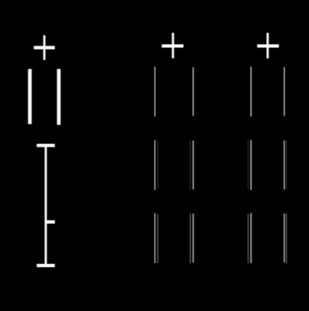
\includegraphics[width=\textwidth]{./Template_Figures/Tsirlin_exp}
        \caption{}\label{fig:tsirlin_exp}
    \end{subfigure}
    \begin{subfigure}[b]{0.5\textwidth}
        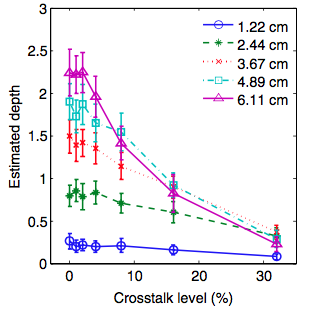
\includegraphics[width=\textwidth]{./Template_Figures/tsirlin_res}
        \caption{}\label{fig:tsirlin_res}
    \end{subfigure}
    \caption{(a) The setup of Tsirlin's experiments. Left side represents the complete experiment where the viewers see the vertical lines as a single line in depth. The right side shows the same line with 0, 16 and 32\% simulated crosstalk. (b) Depth degradation averaged over the test subjects.\label{fig:tsirlin}}
\end{figure}
They observed that the perceived depth decreased with the increase in crosstalk as well as increase in disparity. In the second part of the experiment, they observed the effect of crosstalk on binocular occlusion and found out that effect of crosstalk on the perceived depth due to occlusion was even more swear. In 2012 \cite{tsirlin2012effect}, they performed similar experiments to observe the effects of crosstalk on thin structures where the ghost is always completely separated from the stimulus (which is usually the case with vertical thin structures present at a significant distance from the plane of focus). Again they found that observed depth degrades significantly as the disparity or the crosstalk level was increased. However this time the degradation was observed to be higher than the case where the ghosts always overlapped the stimulus. One problem with these experiments is that the stimuli are presented as a uniformly luminant objects on a black background where there is no other depth cue present. This is usually not the case with the complex scene that we typically observe in 3D movies. We observed in our test experiments that in such monochromatic scenes, the depth of the stimuli was extremely hard to perceive even at moderately high disparities. Tsirlin also observed that the perceived depth degraded with disparity even in the base case i.e. the case where crosstalk was set to zero. This is not usually the case in complex scenes. Secondly, there was no reference used and the subjects were simply asked to report the observed depth via a slider bar that was controlled with a mouse. This `rating' setup can be problematic because it can not be guaranteed that all the subjects would rate the same depth equally. And finally, the relation of the stimulus width to the perceived depth at different disparities was not determined which we think is also necessary.

Tsirlin et al \cite{tsirlin2012crosstalk} again performed similar experiments but this time with complex natural scenes. The subjects were shown a complex scenes with the objects of interest marked by arrows. Later, they were shown the exact same images with crosstalk induced and were asked to rate the depth difference they observed between those two objects. The results again concluded that the perceived depth difference decreased as the theoretical depth difference between the objects of interest and the crosstalk increased. One problem with this experiment is that it reports the observed depth in a complex cluttered scene where the ghosts from the neighboring objects will play a significant role in determining the observed depth difference. Hence it does not tell us anything about how the HVS will respond to the geometry of the stimulus. Moreover, the users rating can be deviated from each other.

\section{Depth resolution mechanisms in HVS}
% \subsection{Banks and cormacks work}
It is clear that crosstalk in stereoscopic displays reduce the perceived depth proportional to the level of crosstalk and the disparity of an object. However, in order to understand why the perceived depth is degraded, we had to look into some literature where the depth information extraction by the HVS from disparity is investigated.

It is widely believed that the HVS uses some kind of cross-correlation of retinal patches between the two eyes in order to determine the location (or in other words the disparity) at which some object is located in a retinal image with respect to the other. Cormack \cite{cormack1991interocular} investigated the binocular fusion process with respect to contrast of the stimuli and concluded that the binocular fusion was dependent upon the contrast and the strength of the binocular cross-correlation profile of the stimuli. The cross-correlation was computed as a function of image luminance. The stimuli used in his experiments were random dot stereograms in which the number of white dots matching between the left and the right eye images at some disparity represented the interocular correlation. He concluded that at low contrast, the binocular fusion increased when the contrast of the stimuli (white dots in the stereograms) increased. The reason behind this can be seen in figure \ref{fig:cormack_cont} where the cross-correlation (interocular correlation IOC \index{IOC}) profiles at different contrasts has been plotted. The peaks in these profiles represents the disparity at which the two images matched the most. It is clear that as the contrast decreases, the distinctness of the these peaks also degrades which might make it difficult for the HVS to identify. Same is also true if noise is added to the images as seen in figure \ref{fig:cormack_noise}. This can be one of the reasons for the degradation of the perceived depth in ghosted images as the ghost (due to crosstalk) in an image is just a low contrast version of the stimulus added into the image at some disparity effectively reducing the local contrast. We used these finding in deriving our own model for the HVS that will be explained in chapter 5.

\begin{figure}[htbp]
    % \centering
    \begin{subfigure}[b]{0.5\textwidth}
        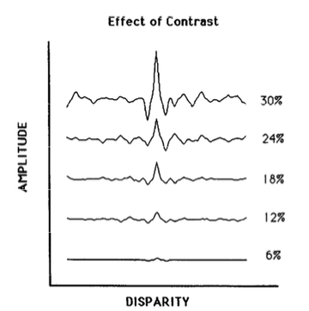
\includegraphics[width=\textwidth]{./Template_Figures/cormack_cont}
        \caption{}\label{fig:cormack_cont}
    \end{subfigure}
    \begin{subfigure}[b]{0.5\textwidth}
        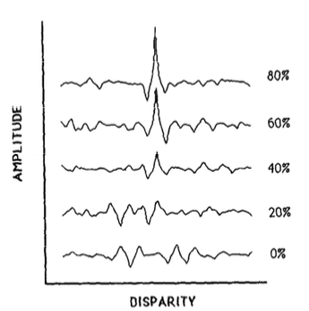
\includegraphics[width=\textwidth]{./Template_Figures/cormack_noise}
        \caption{}\label{fig:cormack_noise}
    \end{subfigure}
    \caption{(a) 1D cross-correlation with varying contrast. (b) 1D cross-correlation with variable level of added noise.\label{fig:cormack}}
\end{figure}

Filippini and Banks \cite{filippini2009limits} explained the limits of stereopsis and modeled them by using windowed interocular cross-correlation. The neighborhood of each pixel in one stereo images (say left) was weighed by an isotropic Gaussian window followed by horizontally displacing a similar window in the right eye image. For each displacement, the cross-correlation of the windowed patched was computed. The disparity was obtained at the displacement value where the maximum correlation for the patches was obtained. The 2D cross-correlation formula used was as seen in equation \ref{eq:ccr}.
\begin{equation}
c(\delta_x) = \frac{ \sum\limits_{(x,y) \in W_L} [(L(x,y) - \mu_L)(R(x-\delta_x, y) - \mu_R)] }{\sqrt{\sum\limits_{(x,y) \in W_L}(L(x,y) - \mu_L)^2} \sqrt{\sum\limits_{(x,y) \in W_R}(R(x-\delta_x, y)- \mu_R)^2}}
\label{eq:ccr}
\end{equation}
Where L(x,y) and R(x,y) are the image intensities for the left and right eye, W\textsubscript{L} and W\textsubscript{R} are the Gaussian windows applied to the images, $\mu\textsubscript{L}$ and $\mu\textsubscript{R}$ are the mean intensities within the two windows, and $\delta_x$ is the displacement (disparity) of window W\textsubscript{R} relative to W\textsubscript{L}. This way, the correct disparity for each object in stereo images can be computed. The problem is that this method also computes the correct non-degraded disparity even if the crosstalk is induced to the images. This does not correspond well to the HVS behavior. Hence we need an HVS model that can simulate not only the correct disparity estimation but also the degraded disparity when crosstalk is added to the images. \textcolor{red}{note  to self: Mention the disparity gradient as explained in this paper in the discussion.}

\section{Reduction of crosstalk}

As mentioned in the previous sections, crosstalk severely hinders the perceived depth and reduces the overall visual quality and viewer comfort. Hence it is imperative for the crosstalk levels to be mitigated or at least lowered to an unperceivable level. Almost all of the 3D displays using present hardware technologies have some amount of crosstalk present in them. Fortunately it is possible to calculate the amount of leakage between views at any position for any display. Usually a luminance meter is used to detect the amount of light leaked between views. Once the leakage levels for a display system are computed, image processing techniques can used to preprocess the stereo images in such a way that results in mitigation or minimization of the perceived ghosting once they are displayed on any traditional 3D screen.Early attempts relied on subtracting from one view image, the leaked image intensity from other perspective view before displaying. This technique might result in  negative light intensities in low contrast areas of the images. Since negative light can not be produced by any display, the areas of the preprocessed image that has negative intensities are clamped to zero. Which means that the crosstalk in these areas is not fully subtracted and hence the ghosting still persists. One way to avoid such problem is to increase the overall image intensity by some value such that no negative values are obtained after crosstalk subtraction. This however comes at a cost of decreased average contrast of an image hence degrading the overall image quality. In the following sections we will review some of the contemporary techniques that are used in order to remove the crosstalk as well as maintaining the overall image quality.

\subsection{Stereoscopic screens}

 Konard et al \cite{konrad2000cancellation} proposed a crosstalk reduction technique that took the ghosting perception thresholds into consideration.For every possible combination of crosstalk level and the contrast of the scene, they experimentally computed the minimum level of light intensity that after subtraction would bring the ghosting to an undetectable level by a human observer. Ghosting was later minimized efficiently by storing and using these values from a lookup table. In order to avoid the negative light intensity values after crosstalk subtraction, they proposed to increase all the pixel values by the maximum negative intensity obtained hence reducing the overall image contrast. Limpscomb and Wooten \cite{lipscomb1994reducing} took the specially non-uniform nature of crosstalk in the display into consideration and proposed a technique that consisted of dividing the screen into 16 horizontal bands. The crosstalk was evaluated for each of these bands followed by the crosstalk subtraction in the images accordingly. The problem with this technique is that the non uniformity of the crosstalk level between and across the bands is continuous in nature which is why it resulted in over and under subtraction of crosstalk between bands that was still perceivable by the viewers. Another problem is that all of the above mentioned techniques assumes static scenes and hence ignore the temporal aspects. In a time sequential displays, crosstalk is induced not only by the view image from the opposite aspect (i.e. left and right view) but also from the views in the previous frame. Smit et al \cite{smit2007non} took this phenomenon into consideration as well. However, as the problem with every subtractive approach, this technique also suffered from the over subtraction. Sohn and Jung \cite{sohn2014crosstalk} proposed a technique that utilized disparity adjustments for a scene such that the least amount of uncorrectable crosstalk occurs in perceptually important regions. A crosstalk visibility estimator that simulated human sensitivity to luminance changes according to Webber's law was used in order to determine the areas in a scene where the spatio-temporal crosstalk was visible. In the second step, the global disparities in the scene were changed (shifting the zero plane) and the amount of perceivable uncorrectable crosstalk was computed using the crosstalk visibility estimator for every step. The global disparity shift that yielded the lowest amount of uncorrectable visually important crosstalk was chosen for displaying. In order to remove the already minimized uncorrectable crosstalk, the intensities in the scenes was locally increased in order to preserve as much dynamic range as possible.

\begin{figure}
\centering
    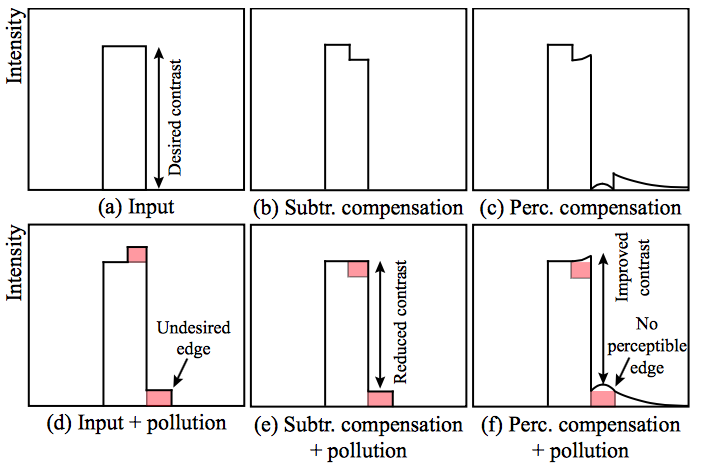
\includegraphics[width=0.7\textwidth]{./Template_Figures/perceptual_ct}
    \caption{(a) Input image. (b) Subtractive compensation. (c) CSF weighed compensation. (d-f) Observed images \cite{van2011perceptually}.\label{fig:perc_opt}}
\end{figure}
 Most recently, Baar and Poulakos et at \cite{van2011perceptually} proposed a crosstalk reduction minimization that utilized the contrast sensitivity function CSF\index{CSF} to steer the minimization in such a way that only perceptually important areas in a scene are corrected.
 \begin{equation}
\underset{x}{\operatorname{argmin}}||\lambda_l \: . \: r||^2, \:\:\: s.t. \:\:\: 0 \leq x \leq 1.
\label{eq:perc_opt}
\end{equation}
\begin{equation}
r\: = \: x\: + \: \phi(x)\: - \: \bar{x}
\label{eq:residual_eq}
\end{equation}
where $\lambda_l$ is a diagonal matrix of the CSF spectral coefficients, x and $\bar{x}$ denotes the original and the compensated images respectively and $\phi()$ denotes the non-linear function representing the crosstalk. The constraints on the optimization are necessary so that the minimized image values does not exceed the displayable range. Using the CSF helps spread the intensities of the uncorrectable crosstalk to the areas which are perceptually less important (as seen in figure \ref{fig:perc_opt}). Also in this figure, it can be seen that the optimization introduces a cornsweet profile at the edges effectively improving the local contrast. One other factor that is important for the perception is visual masking i.e. the phenomenon where a signal is undetectable in presence of another signal with similar pattern. Baar and Poulakos further improved the optimization by incorporating into equation \ref{eq:perc_opt} an additional weighing with visual masking operator.
\begin{equation}
\underset{x}{\operatorname{argmin}}||\lambda_n\:.\:\lambda_l \: . \: r||^2, \:\:\: s.t. \:\:\: 0 \leq x \leq 1.
\label{eq:perc_opt_vm}
\end{equation}
Here $\lambda_n$ is a visual masking binary operator that will help ignoring the optimization for non-perceivable areas of the ghosted image due to visual masking. This idea can also be used for optimization of light fields in automultiscopic displays.

\subsection{Automultiscopic screens}
As discussed in chapter 2, crosstalk in an automultiscopic screen is introduced by the neighboring views i.e. the horizontal neighbors of a pixel in case the lenticular sheet is not tilted as well as the vertical neighbors of the same view in case the lenticular sheet is tilted. This is because a tilted sheet can not cover a whole pixel of the underlying LCD panel completely. Due to this reason, eliminating crosstalk from automultiscopic displays is trickier than stereoscopic displays.

Barkowsky and Campisi \cite{barkowsky2010crosstalk} proposed that for each view of an automultiscopic display, the ghosting from within and across the views can be observed and composed as coefficients of a circulant Toeplitz matrix. Hence for an automultiscopic screen with 8 views, the perceived views can be modeled as
\begin{equation}
L_p = (E\:+\:A)\:.\:L_d
\label{eq:perc_view}
\end{equation}
where $L_p$ and $L_d$ are the vectors of displayed and perceived images in luminance domain, A is the circulant Toeplitz matrix approximating the crosstalk coefficients and E is 8x8 identity matrix. A generic reduction of crosstalk was derived from equation \ref{eq:perc_view} for each channel
\begin{equation}
L_{rd} = (E\:+\:A)^{-1}\:.\:L_{ri}
\label{eq:ct_red_red}
\end{equation}
where $L_{ri}$ is the gamma corrected intended luminance of the red channel. The implementation of this will generate luminance values that are beyond the range of the display (negative values) hence equation \ref{eq:ct_red_red} can be modified in order to increase the average contrast of the image.
\begin{equation}
L_{rd} = (E\:+\:A)^{-1}\:.\:\left(\frac{r_i.(255-\beta)+255.\beta}{255^2}\right)^{\gamma}
\label{eq:ct_red_reduced_contrast}
\end{equation}
here the term $\beta$ denotes the level to which the black level must be shifted up. As expected, this will avoid getting any negative values for luminance but decrease the image contrast. The authors claimed that a certain level of negative values can be tolerated hence for each view, the value of beta was computed iteratively that resulted in no more than a desired number of negative values.

Since the light leakage from neighboring left and right views can be considered as non energy preserving blurring, inverse filtering might be applied to the images in order to minimize the perceivable ghosting. Jain and Konard \cite{jain2007crosstalk} derived a blurring filter that simulated the light leakage from the neighboring views, combined it with the anti-aliasing filter typically used in automultiscopic displays and used Weiner inverse filtering to preprocess the images in order to mitigate the crosstalk. Li \cite{citation-0} argued that light leakage from the same view due to incorrect sub-pixel approximation is more severe than light leakage from the neighboring views and hence proposed to use an appropriate filter that mimics the sub-pixel light leakage in order to be used for inverse filtering.

Generally, the simulation of crosstalk can be written as a system of equations AX=B where A is the crosstalk coefficient matrix as described above, X is the set of intended images and B is the set of crosstalk added view images. Naively, one can compute crosstalk free X by solving $X=A^{-1}B$. However, for this to work, A should be a full rank matrix and even then the result will be unacceptable since the resulting preprocessed images will contain negative values. Wang and Hou \cite{wang2014improved} first proposed a mathematical model for computing the crosstalk coefficient matrix A only by using the parameters of the screen such as screen resolution, pixel dimensions, and the angle of the tilt of lenticular sheet. They argued that usually the crosstalk is measured experimentally which is always prone to errors. The mathematical model should provide a more reliable crosstalk estimation. Secondly, they proposed solving this linear system of equations in a constrained manner where the values of X can not exceed the range [0,255]. They named it as Box-Constrained Integer Least Square (BILS) solution.
\begin{equation}
\begin{aligned}
\underset{X \in BOX_x}{\operatorname{min}}||B\: -\: AX||_2^2 \\
BOX_x\: = \: {X\: \in \: \mathbb{Z}^{w*h} \: : \: L\: \leq \: X\: \leq\: U }
\end{aligned}
\label{eq:bils}
\end{equation}
where $||.||_2$ denotes the Euclidean norm, w and h are the width and height of the screen resolution, and L and U are vectors of 0 and 1 respectively.